\documentclass[../Main.tex]{subfiles}

\begin{document}
\subsection{Browser Page}
This is the basic view of the browser, here you can navigate around the web, check resonse statuses and view the pages source code.
\begin{figure}[H]
    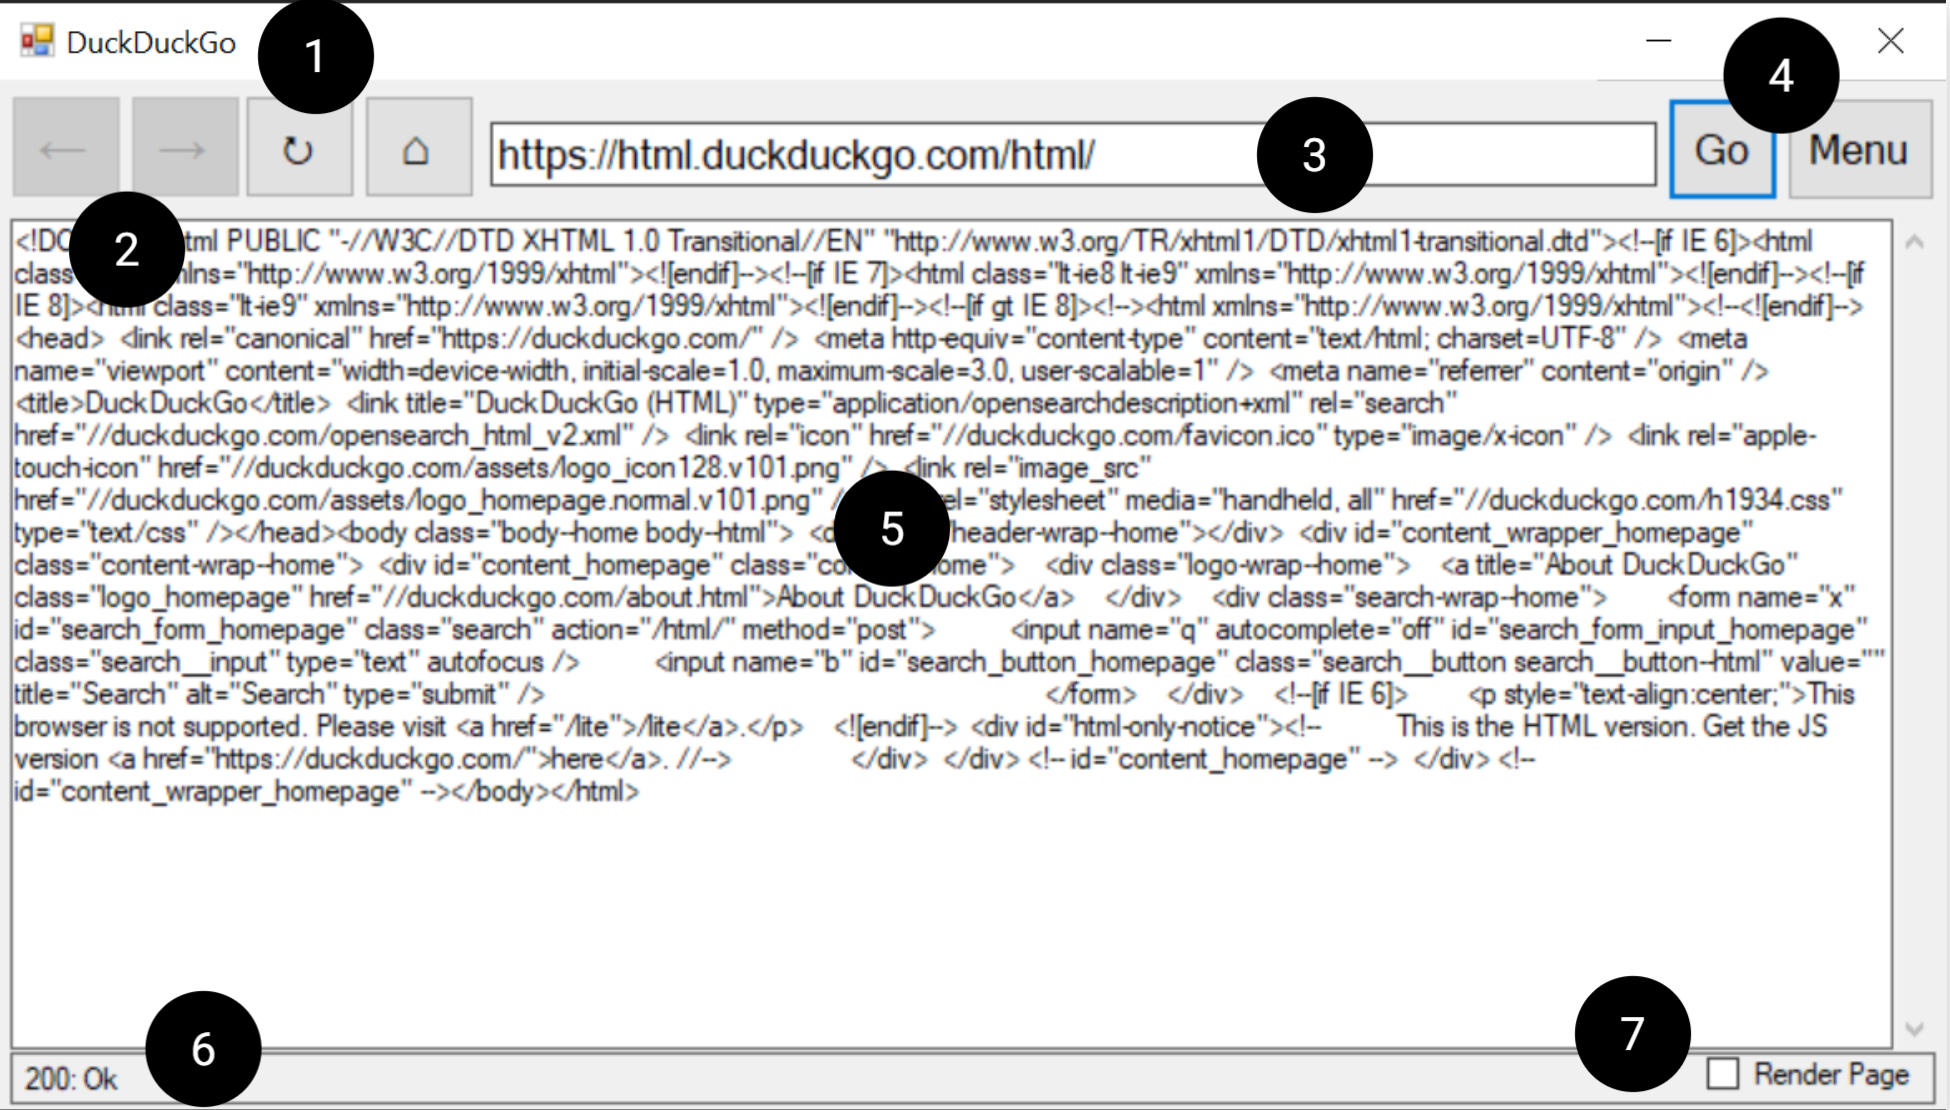
\includegraphics[width=1\textwidth]{BasicViewAnnotated.png}
    \caption{Basic browser view}
    \label{fig:BasicView}
\end{figure}
\begin{enumerate}
    \item Web Page title
    \item back, forwards, refresh \& home buttons - Standard, familiar browser navigation buttons
    \item URL text input box - Input desired URL here
    \item Go \& Menu buttons - click Go to navigate to the URL contained in the text box
    \item HTML source code view
    \item HTTP status code / message
    \item Render page toggle check box - Check this to toggle to a rendered view of the page
\end{enumerate}

\subsection{Menu expanded}
Fig.~\ref{fig:MenuExpanded} shows the menu open, options for setting the home page, adding to favourites, adding custom favourites, viewing the history/favourites are within this menu.
\begin{figure}[H]
    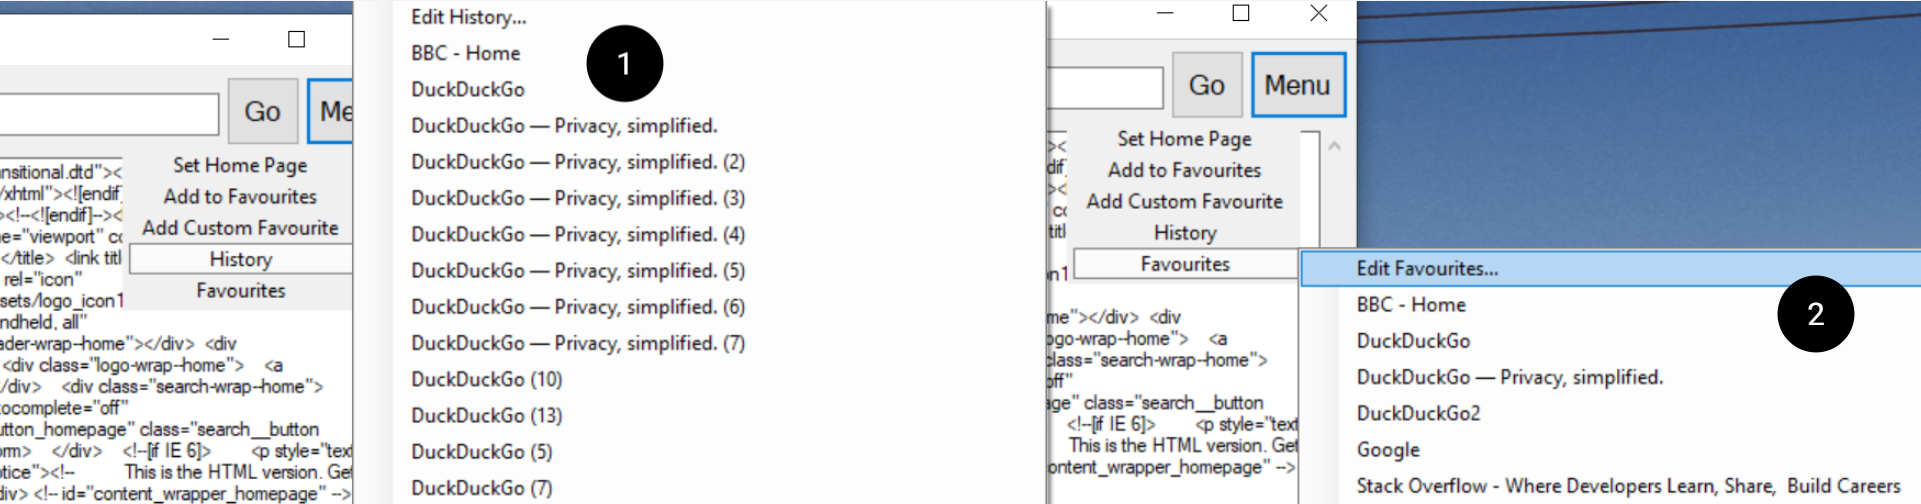
\includegraphics[width=1\textwidth]{HistoryFavMenuAnnot.png}
    \caption{Menus opened}
    \label{fig:MenuExpanded}
\end{figure}

\begin{enumerate}
    \item This is the opened menu with History selected, you can select any one of these elements and navigate to the page.
    \item This is the Favourites menu opened, highlighted is `Edit Favourites...' clicking this will open the favourites editor window.
\end{enumerate}

\subsection{Edit Favourites}
Fig.~\ref{fig:EditFavourite} shows the window that opens upon selecting the edit favourites button in the menu.
\begin{figure}[H]
    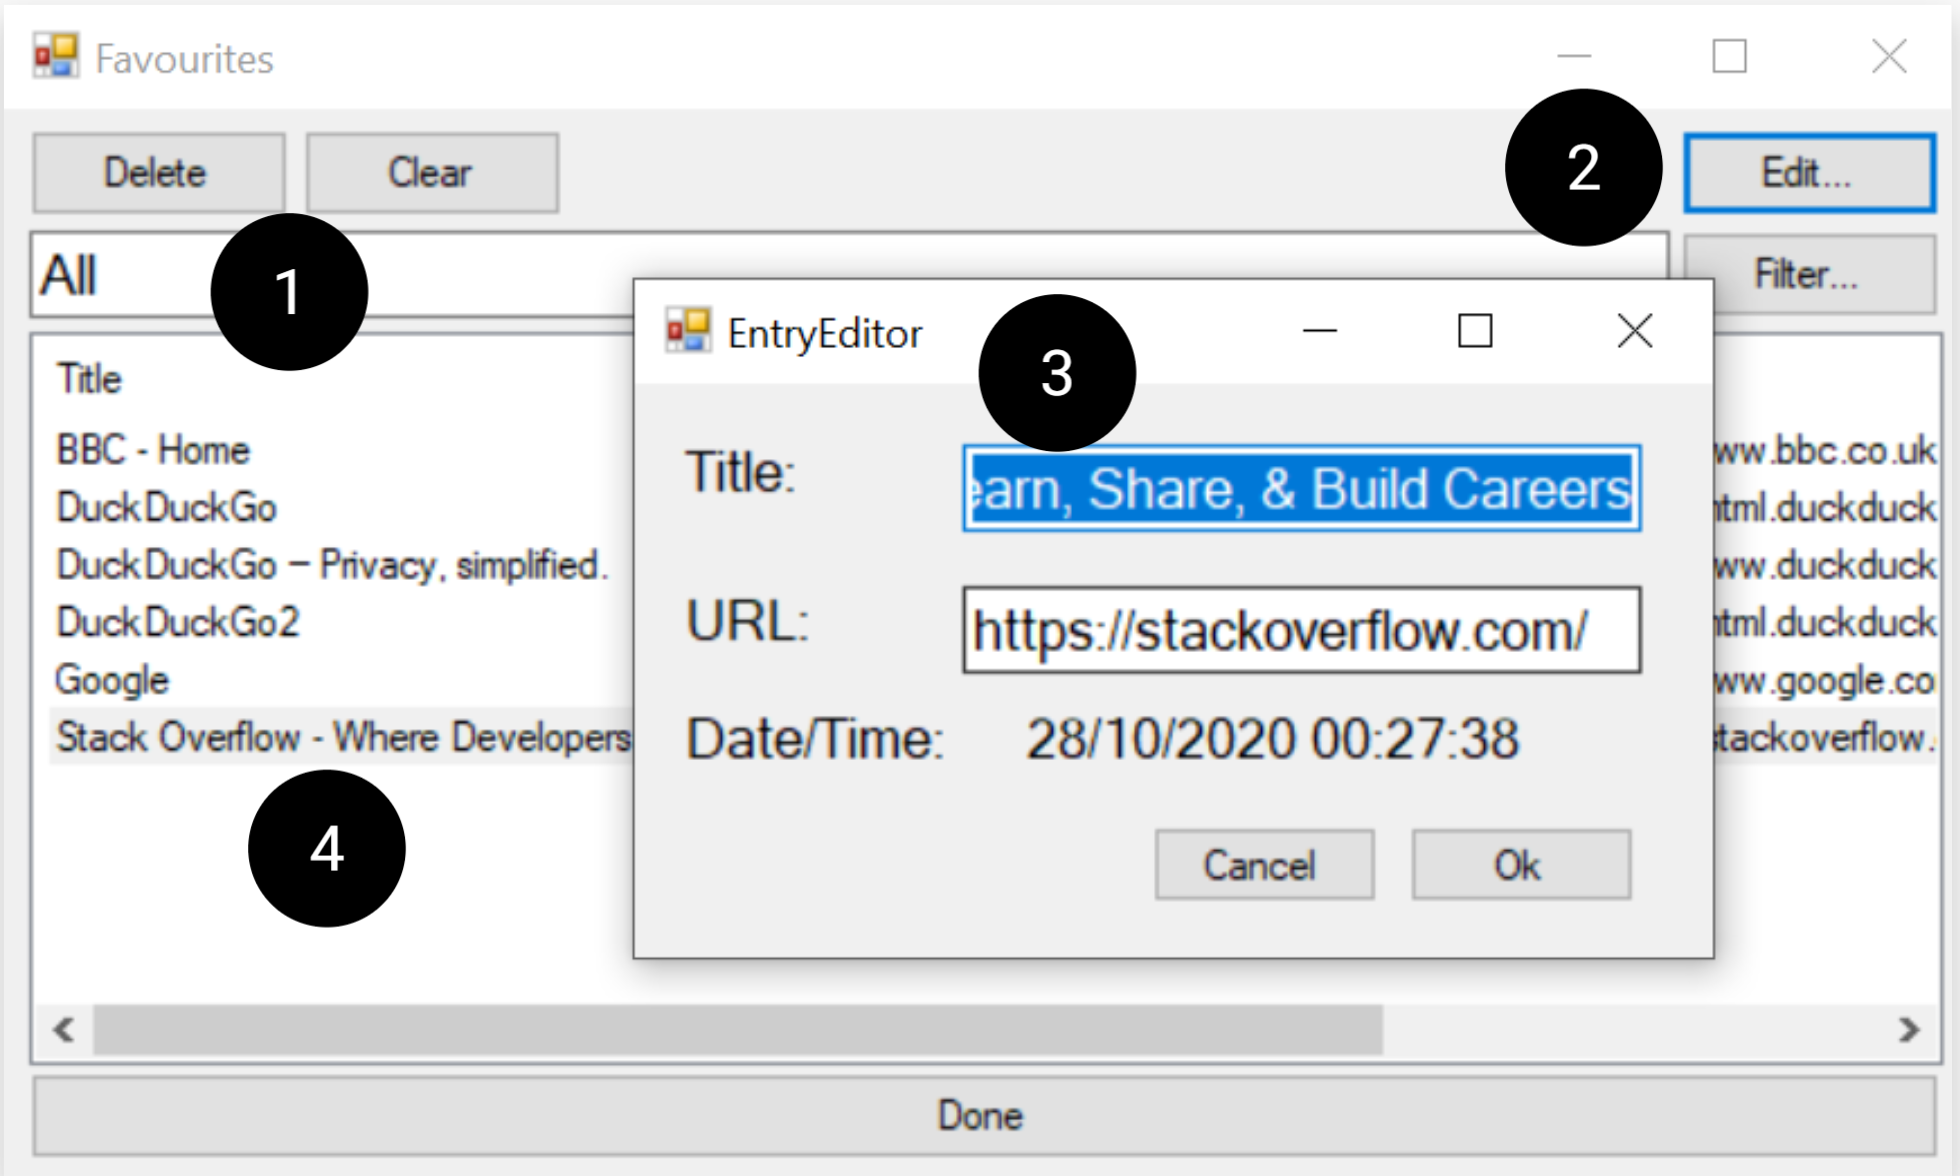
\includegraphics[width=1\textwidth]{EditFavAnnotated.png}
    \caption{Editing a favourite}
    \label{fig:EditFavourite}
\end{figure}

\begin{enumerate}
    \item Here you can see the delete and clear buttons, along side a filter text box(non-functional)
    \item This is the edit button, this is only avaliable when a single item in the list of elements is selected
    \item The Entry Editor window lets you modify the Title or URL of the entry but changing the contents of the text boxes
    \item Here we can see a list of all the current favourites, their titles, urls, and access times.
\end{enumerate}

\end{document}
